\begin{appxchp}
\appxtle{附录样式示例}
这是《手册》27页的附录A示例。

引用示例:如图~\ref{appxfig:appxexampleA}

\begin{figure}[htbp]
\begin{center}
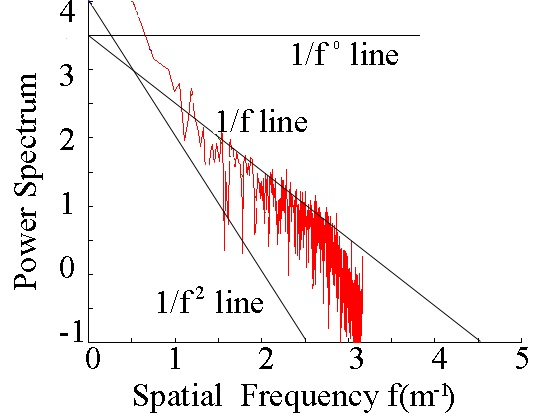
\includegraphics[width=0.9\linewidth]{fulu1.jpg}
\end{center}
\appxfig{频谱图}
\label{appxfig:appxexampleA}
\end{figure}

\end{appxchp}

\begin{appxchp}
\appxtle{图片、表格、公式示例}
这是前面内容的复制粘贴,目的在于附录样式的展示

\begin{figure}[htbp]
\centering
\subfloat[分布符合1/f规律图]{%

\includegraphics[height=40.8mm]{3.png}}\hspace{4em}%
\subfloat[大小与色彩符合1/f规律图]{%
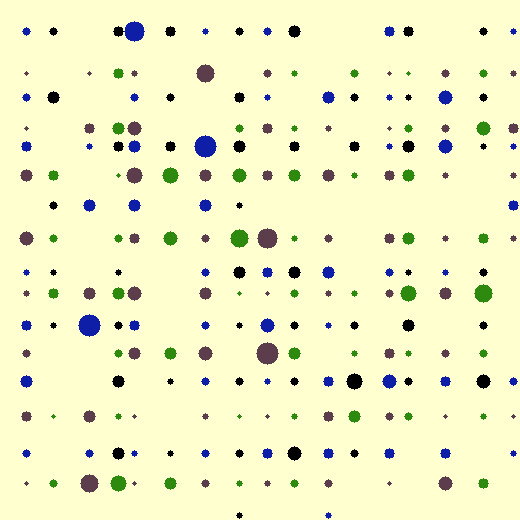
\includegraphics[height=38.4mm]{4.png}}\hspace{4em}
\subfloat[间距、大小与色彩均符合1/f规律图]{%

\includegraphics[height=41.7mm]{5.jpg}}
\appxfig{图案例}
\end{figure}

\begin{table}[htbp]
\appxtab{并排子表格}
\begin{center}
\subfloat[第一个子表格]{
\begin{tabularx}{0.3\linewidth}{Z|Z}\toprule
111 & 222 \\\midrule
222 & 333 \\\bottomrule
\end{tabularx}}\hspace{0.15\linewidth}
\subfloat[第二个子表格]{
\begin{tabularx}{0.3\linewidth}{Z|Z}\toprule
111 & 222 \\\midrule
222 & 333 \\\bottomrule
\end{tabularx}}
\end{center}
\end{table}

附录中的公式不需要加编号,所以记得使用无编号的公式环境。

\begin{equation*} 
\left(\begin{array}{c|c} 
1 & 2 \\ 
\hline 3 & 4 \end{array}\right) 
\end{equation*}   

\begin{eqnarray*}
f(x) & = & \cos x \\ 
f'(x) & = & -\sin x \\ 
\int_{0}^{x} f(y)\,dy & = & \sin x 
\end{eqnarray*} 

\begin{eqnarray*} 
\sin x & = & x -\frac{x^{3}}{3!} +\frac{x^{5}}{5!}-{} \nonumber\\ 
	& & {}-\frac{x^{7}}{7!}+{}\cdots 
\end{eqnarray*}

\end{appxchp}